\documentclass[11pt,a4paper]{report}

\usepackage[english]{babel} 
\usepackage[utf8]{inputenc} % Unicode
\usepackage{graphicx} 
\usepackage{url} 
\usepackage{amsmath}
\usepackage{textcomp} 
\usepackage{multirow} 
\usepackage[pdftex,hidelinks]{hyperref}
\usepackage{listings}
\usepackage{natbib}
\usepackage{graphicx}
\usepackage{hyperref}
\usepackage{verbatim}
\usepackage{acronym}
\usepackage{ textcomp }

\def\R{{\textsl{R }}}
\def\Shiny{\textsl{Shiny }}
\def\sar{\textsl{SARS-CoV-2 }}



\title{Development of a \Shiny application to visualize SARS-CoV-2 vaccination data of Portugal}

\author{
  Bruna Araújo\\
  \texttt{A84408}
  \and
  Matias Capitão\\
  \texttt{A82726} \\ 
  \\ Mentoring:\\
  Stora Cecília \\
  \and
  Rafael Antunes\\
  \texttt{A77457}
}
\date{May or June 2021}



\begin{document}

\maketitle

\begin{abstract}
% Apagar daqui
    ************* Ao fim retornamos aqui.\\ Entretanto encontrei isto para nos ajudar a fazer o Abstract *************\\ \\
%até aqui
    Write the abstract at the very end, when you’ve completed the rest of the text. There are four things you need to include:\\ \\

    Your research problem and objectives\\
    Your methods\\
    Your key results or arguments\\
    Your conclusion

\end{abstract}

\tableofcontents
\newpage

\listoffigures
\newpage

\listoftables
\newpage

{\huge\textbf{Acronym List}}\\
\begin{acronym}[MPC] % Give the longest label here so that the list is nicely aligned
\acro{IDE}{Integrated Development Environment}
\acro{WHO}{World Healh Organization}
\acro{EU}{European Union}
\acro{ECDC}{European Centre for Disease Prevention and Control}

\end{acronym}


\chapter{Introduction}
\section{\R and \Shiny}

\textbf{\R}  is a program created in 1993 by Ross Ihaka and Robert Gentleman  defined as
"a language and environment for statistical computing and graphics" \cite{R-project website}.
\\
 RStudio is an integrated development environment (IDE) for R. \cite{rstudio}
\begin{figure}
\centering
\begin{subfigure}{.5\textwidth}
  \centering
  
\includegraphics[width=3cm]{images/R.jpg}
  \label{fig:sub1}
\end{subfigure}%
\begin{subfigure}{.5\textwidth}
  \centering
  
\includegraphics[width=5cm]{images/Rstudio.png}
  \label{fig:sub2}
\end{subfigure}
\caption{Logos of R and RStudio}
\label{fig:test}
\end{figure}
\\
R has over 10,000 packages in the CRAN repository which are constantly growing. 
\textbf{\Shiny} is an \R package that makes easy to build interactive web applications \cite{shiny} .
\\
With this package we can combine the computational power of \R with the versatility and interactivity of modern web. This feature it's relevant to develop plots and graphics that can be understood by everyone, and looking pretty while doing it.



% Apagar aqui
\\
\\
\textbf{NÃO GOSTO DESTA ULTIMA FRASE. DESPOIS VER ESTA CENA.}

%Até aqui

\section{SARS-CoV-2}
\subsection{Brief description}



\sar is the name of the coronavirus that caused the current COVID-19 pandemic. According to \ac{WHO}, the first human cases of COVID-19, were first reported from Wuhan City, China, in December 2019. 
The main symptoms of Covid-19 are fever, cough, breathing difficulties, loss of smell and taste. 
It's a disease that attacks all age levels and is transmitted mainly by air, via particles that we expel. \\
There are several reasons for the pandemic to spread globally, mainly the fact that a patient may be asymptomatic, which can cause him to transmit the virus without knowing it. For the same reason, the fact that the incubation period is about 14 days is also a factor to be taken into account. 

\subsection{Vaccination}
Vaccines are substances made up of pathogens (viruses or bacteria), living or dead, or their derivatives. They stimulate the immune system to produce antibodies that act against pathogens that cause infections.

Vaccination is a way to protect people from harmful diseases. It uses the body's natural defenses to build resistance to specific infections and makes the
 stronger immune system.
It reduces the possibility of contracting the disease and thus prevents it from spreading.
\\
As soon as the COVID-19 pandemic took hold in the world, research for the production of safe and effective vaccines began immediately. Vaccination is critical to ending the COVID-19 pandemic. WHO is working tirelessly with partners to develop, manufacture and distribute safe and effective vaccines.
\\
Until May 10, 13 vaccines have been authorized by at least one national regulatory authority for public use. However, in Europe, after consulting the list of authorized vaccines on the \cite {EU} official website of the \ac{EU}, we have four vaccines available: 
\begin{itemize}
    \item BioNTech-Pfizer - (2020/12/21)
    \item Moderna - (2021/01/06)
    \item AstraZeneca - (2021/01/29)
    \item Johnson \& Johnson - (2021/03/11)
\end{itemize}
But it's not the vaccines that will stop the pandemic, it's the vaccination. 
\\





\section{Portugal}

\subsection{Brief description}
Portugal is a country in Europe with a resident population of around 10.2 million inhabitants.  \\
According to the local statistics institute, INE (Instituto Nacional de Estatística - National Statistics Institute), in the publication dated 2019 and edited in 2020, called \cite{pubINE}"Demographic Statistics - 2019", we can find some interesting information such as:
\begin{itemize}
    \item In percentage terms, relative to \textbf{sex},
    \begin{itemize}
        \item \textbf{47,2\textdiscount} of the population is \textbf{male};
        \item \textbf{52,8 \textdiscount} of the population is \textbf{female}.
    \end{itemize}  
    \item In terms of \textbf{age} percentages, 
    \begin{itemize}
        \item \textbf{13,6\textdiscount} of \textbf{young people} (0-14 y/o);
        \item \textbf{64.3\textdiscount} of people of \textbf{working age} (15-64 y/o);
        \item \textbf{22.1\textdiscount} of \textbf{elderly people} (65+ y/o). 
    \end{itemize}
\end{itemize}

Se calhar por aqui alguns graficos relativos ao descrito acima nao é má ideia.

\subsection{Regions}
In terms of NUTS II regions, Portugal is divided in seven groups.
The structuring of the Portuguese territory according to the New Territorial Units for Statistical Purposes, NUTS 2013,  in application in the National Statistical System since 1 January 2015 is composed of seven NUTS II: North, Centre, Lisbon Metropolitan Area (AML), Alentejo and Algarve regions, on the mainland, and the two autonomous regions. \cite{INEE}
\begin{figure}[h]
\centering % para centralizarmos a figura
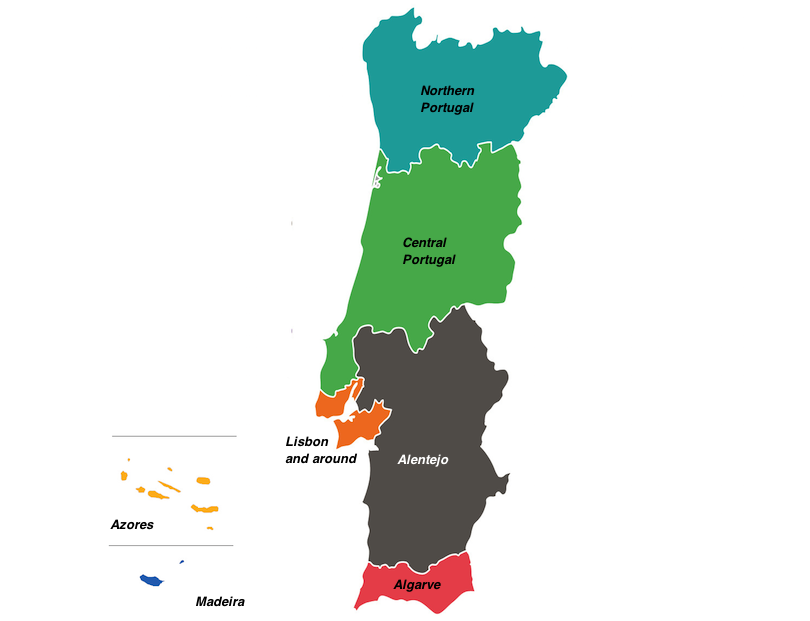
\includegraphics[width=10cm]{images/portugal.png} 

\caption{Portugal's Regions}
\label{figura:qualquernome}
\end{figure}

We'll describing them below, also mentioning some statistical data that may be interesting. \\
All information related to the labor market in the regions was obtained by consulting the  website of the European Commission \cite{trab}. The demographic percentages presented are based on data from  National Institute of Statistics of Portugal, INE. 

\subsubsection{North}
The employment structure in the North region presents 3 sub-regions with specific characteristics: 
The Porto Metropolitan Area, with a strong incidence of services (mainly trade) with greater technological and knowledge intensity. A surrounding shore, where industrial employment is  higher than the national average and rural areas, where nearly half of employment is concentrated in agriculture or non-commercial services.

In terms of {\textbf{demographics}}:
    \begin{itemize}
        \item Population density: {34,73\textdiscount} . 
        \item Gender: {47,2\textdiscount} male and {52,8\textdiscount} female.
        \item Age: 
        \begin{itemize}
        \item {12,63 \textdiscount} aged 14 and younger;
        \item {66,43\textdiscount} aged 15 to 64;
        \item {20,94\textdiscount} aged 65 and older.
        \end{itemize}
    \end{itemize}

\subsubsection{Center}
In this region, the Services sector is the most relevant in terms of employment - with emphasis on Trade and Vehicle Repair, Health and Social Support Services and the Education. \\
In terms of {\textbf{demographics}}:
    \begin{itemize}
        \item Population density: {21,54\textdiscount} . 
        \item Gender: {47,42\textdiscount} male and {52,58\textdiscount} female.
        \item Age: 
        \begin{itemize}
        \item {12,05 \textdiscount} aged 14 and younger;
        \item {63,42\textdiscount} aged 15 to 64;
        \item {24,53\textdiscount} aged 65 and older.
        \end{itemize}
    \end{itemize}
    
\subsubsection{Metropolitan area of Lisbon }
This is the region with the highest population density in the country. It's the region with the highest concentration of services, with emphasis on services provided mostly by the Public Sector; Education; Health and social support services.\\
In terms of {\textbf{demographics}}:
    \begin{itemize}
        \item Population density: {27,81\textdiscount} . 
        \item Gender: {46,71\textdiscount} male and {53,29\textdiscount} female.
        \item Age: 
        \begin{itemize}
        \item {15,88\textdiscount} aged 14 and younger;
        \item {62,04\textdiscount} aged 15 to 64;
        \item {22,08\textdiscount} aged 65 and older.
        \end{itemize}
    \end{itemize}
    
\subsubsection{Alentejo}
This is the region with the lowest population density in the country. Most of the region's territory is dedicated to Agriculture, allied to cattle breeding and also forestry.\\
In terms of {\textbf{demographics}}:

    \begin{itemize}
        \item Population density: {6,84\textdiscount} . 
        \item Gender: {47,97\textdiscount} male and {52,03\textdiscount} female.
        \item Age: 
        \begin{itemize}
        \item {12,4\textdiscount} aged 14 and younger;
        \item {62,05\textdiscount} aged 15 to 64;
        \item {25,55\textdiscount} aged 65 and older.
        \end{itemize}
    \end{itemize}
    
\subsubsection{Algarve}
The economic structure of this region is based on 5 strategic sectors associated with the region's natural resources: hospitality, catering and tourism, health, creative activities, agri-food and maritime activities. 
In terms of {\textbf{demographics}}:
    \begin{itemize}
        \item Population density: {34,73\textdiscount} . 
        \item Gender: {47,2\textdiscount} male and {52,8\textdiscount} female.
        \item Age: 
        \begin{itemize}
        \item {12,63\textdiscount} aged 14 and younger;
        \item {66,43\textdiscount} aged 15 to 64;
        \item {20,94\textdiscount} aged 65 and older.
        \end{itemize}
    \end{itemize}
    
\subsubsection{Azores autonomous region}
The region's economy is fundamentally based on activities mainly from the Public Sector (Public Administration, Social Security, Education, Health and Social Support activities). The activities of Trade and Repair of Vehicles and Accommodation and Restoration are equally important in employment in the region. \\
In terms of {\textbf{demographics}}:
    \begin{itemize}
        \item Population density: {2,36\textdiscount} . 
        \item Gender: {48,55\textdiscount} male and {51,45\textdiscount} female.
        \item Age: 
        \begin{itemize}
        \item {15,37\textdiscount} aged 14 and younger;
        \item {69,69\textdiscount} aged 15 to 64;
        \item {14,99\textdiscount} aged 65 and older.
        \end{itemize}
    \end{itemize}
    
\subsubsection{Madeira autonomous region }
In terms of more established work areas, this region is very similar to the Azores region. Tourism has an important role for both regions.\\
In terms of {\textbf{demographics}}:
    \begin{itemize}
        \item Population density: {2,47\textdiscount} . 
        \item Gender: {46,67\textdiscount} male and {53,33\textdiscount} female.
        \item Age: 
        \begin{itemize}
        \item {13,11\textdiscount} aged 14 and younger;
        \item {69,91\textdiscount} aged 15 to 64;
        \item {16,98\textdiscount} aged 65 and older.
        \end{itemize}
    \end{itemize}





\section{SARS-CoV-2 in Portugal}
\subsection{Brief description}

SARS-CoV-2 (Severe Acute Respiratory Syndrome coronavirus) is a new type of coronavirus that causes a respiratory disease called coronavirus disease 19, know as COVID-19. It was first detected in December 2019 has quickly spread globally.

Portugal recorded the first confirmed case of COVID-19 on March 2 and the first death occurred
on March 16. Since then we have added more than 800 thousand registered cases and more than 16 thousand deaths.

Portugal was severely affected by COVID-19, being considered, in the middle of January 2021, as the worst country in the world in terms of infection and mortality rates per million inhabitants and the worst country in Europe with the highest average of cases COVID-19 daily reports, with Portugal reaching a maximum of 16432 cases and 303 deaths on 28 January 2020.












\subsection{Vaccination}

   To end this pandemic, a large part of the world needed to be immune to the virus. The safest way to achieve this was through a vaccine, so with the help of investments by companies, governments, international health organizations and university research groups it was possible to develop a series of vaccines including Phyzer, Moderna, Astrazeneca, Johnson & Johnson, among others.

   The first vaccine administered in Portugal was on December 27, 2020. The first vaccine was António Sarmento, 65, director of the Infectious Diseases Service, at Hospital de São João, in Porto and since then more than 2 million doses of vaccine have been administered. Despite the fact that the entire Portuguese population has access to a vaccine, depending on their clear clinical condition, Portugal opted for a vaccination plan divided into 3 phases, that is, priority groups were defined, as they are more vulnerable to COVID-19, as an example health professionals, professionals and residents of residential structures for the elderly and similar institutions, who were part of the first vaccination phase.


\chapter{Application}




\section{Introduction to RStudio}
R is a statistical programming language and a free, open-access program that has gained considerable popularity in several areas of science. R was developed by statisticians George Ross Ihaka and Robert Clifford Gentleman, as a derivation of the statistical programming language S.
For the development of our application we use the RStudio program.

RStudio is a program that allows a more user-friendly working interface to run R. Instead of using the R desktop, which would actually be a simple notepad where we would type the code and then trigger R to read and running this code (or our script), it's more convenient to use a development interface that has a series of facilities that not only improve code visualization, but facilitate package installation, code error monitoring, data visualization and graphics , among other facilities.


RStudio provides most of the necessary and desirable features for a user-friendly graphical interface making it much easier and more productive to use R. Unlike some of the other platforms mentioned above, RStudio is available for other operating systems (Linux and IOS -Mac ) in addition to Windows, being easier and more intuitive to learn, with extensive free documentation on the internet.



\section{Shiny}

The R Shiny framework is an RStudio package that makes it incredibly easy to build interactive web applications with R. A Shiny has the benefit of allowing us to create highly effective reports and data visualizations where the user can explore a set of data.

Shiny apps are divided into two parts: 

\begin{itemize}
    \item server.r
    \item ui.r (UI)
    
\end{itemize}
 % se tiver a der merd* corrijam 
 
 Ui.R stands for User Interface. The UI controls what is displayed on the application page and how components are laid out. This can include text and other markup elements, graphics, widgets that accept user input, or plots.

 The server controls what data will be through the UI. The server will be where you upload and collate the data and then set your options (ie graphics) using input from the UI.

 
Even though we created two separate files for our application, namely server.r and ui.r , shiny supports single file applications. A single file configuration puts both the server and user interface code in a single app.R file, whereas the multiple file configuration puts them in their own separate files. Functionally, these configurations will produce the same app. The multiple file configuration is generally preferred, especially for larger applications, as it usually makes code easier to manage. For smaller apps, the single file configuration is likely a more efficient way to go.
 
\subsection{Connection between user interface and server}
\begin{figure}[h]
\centering % para centralizarmos a figura
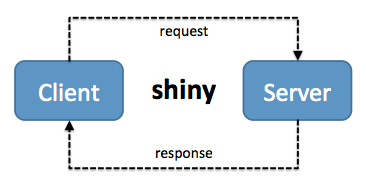
\includegraphics[width=10cm]{images/post-logo.PNG} 

\caption{connection between server and ui}
\label{figura:qualquernome}
\end{figure}
 
In practice, inputs are widgets that enable user interaction with the app. They receive a value chosen by the user and send it to the server side.


ACABAR 








\subsection{Reactivity in shiny}
  In Shiny, you express server logic using reactive programming.
  
  
  The main idea of reactive programming is to specify a dependency graph so that when an input is changed, all related outputs are updated too, for example, we don't need to tell an output to update because due to reactivity the information is always automatically updated, making the flow of an application considerably simpler.
  

   Then reactive functions as it is a way to control which parts of the application are updated, avoiding unnecessary calculations that can make your application slow.

\subsection{Render functions}

The main function for generating documents in R Markdown, from the rmarkdown package, is a render ().
The render () function is a wrapper that internally calls knitr :: knit () and later converts the document to .html using Pandoc, which is a document and open source converter.


A render function that we used in the application was renderPlot (), for example, to display the graphics in our application we use the renderPlot () tool. RenderPlot is a reactive function that can take input data from the ui.R script and feed it into the server.R script.We must use a render* function in the server to tell Shiny how to build your objects. It then actively updates the information within its role.


Thus, the outputs must be built with render() functions, with a render() function for each type of object.




\subsection{Application Format}
  
    
\end{itemize}



\section{Implementation}
\subsection{Depois ver mais cenas}
\section{Results}
\subsection{Publication}
\subsection{Versatility}

\chapter{Conclusion}


\bibliographystyle{plain}
\begin{thebibliography}{10}

\bibitem{R-project website} \textit{\href{https://www.r-project.org/about.html}{https://www.r-project.org/about.html}} , \textbf{About/R-Project website}

\bibitem{shiny}\textit{\href{https://shiny.rstudio.com/l}{https://shiny.rstudio.com}} , \textbf{Shiny website
}
\bibitem{SARS-CoV-2}\textit{\href{https://apps.who.int/iris/bitstream/handle/10665/332197/WHO-2019-nCoV-FAQ-Virus_origin-2020.1-eng.pdf}{https://apps.who.int/.../origin-2020.1-eng.pdf}} ,\textbf{ Origin of SARS-CoV-2 - \ac{WHO}}

\bibitem{EU}\textit{\href{https://ec.europa.eu/info/live-work-travel-eu/coronavirus-response/public-health/eu-vaccines-strategy_pt}{https://ec.europa.eu/info/live-work-travel-eu/coronavirus-response/public-health/eu-vaccines-strategy_pt}} , \textbf{EU vaccine strategy} 

\bibitem{reuters}\textit{\href{https://graphics.reuters.com/world-coronavirus-tracker-and-maps/vaccination-rollout-and-access/}{https://graphics.reuters.com/world-coronavirus-tracker-and-maps/vaccination-rollout-and-access/}}, \textbf{Covid-19 vaccination tracker, Reuters} 


\bibitem{pubINE}\textit{\href{https://www.ine.pt/xurl/pub/71882686}{https://www.ine.pt/xurl/pub/71882686}}, \textbf{Instituto Nacional de Estatística - Estatísticas Demográficas : 2019. Lisboa : INE, 2020.} 


\bibitem{trab}\textit{\href{https://ec.europa.eu/eures/main.jsp?acro=lmi&lang=pt&countryId=PT&catId=57&parentId=0}{https://ec.europa.eu/eures/main.jsp?acro=lmi&lang=pt&countryId=PT&catId=57&parentId=0}}, \textbf{Labor Market Information - European Commission} 



\end{thebibliography}

https://rpubs.com/cassiorampinelli/488999
https://laderast.github.io/gradual_shiny/app-1-connecting-ui-and-server.html#more-about-inputs-and-outputs
https://mastering-shiny.org/basic-reactivity.html











\end{document}

